\section{Approach}
\label{sec:approach}

%\begin{figure}[th]
%\centering
%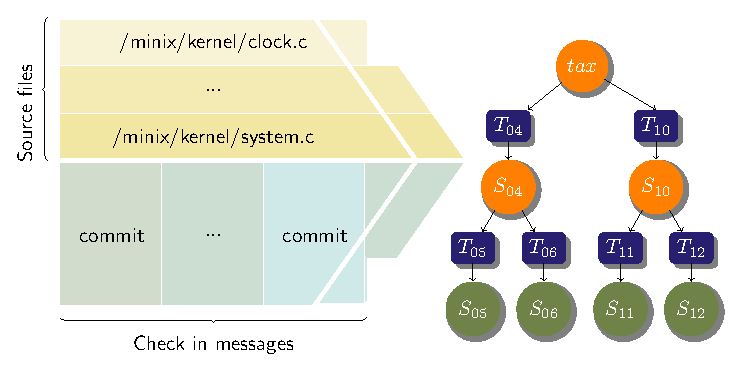
\includegraphics[width=0.8\columnwidth]{picture/framework.eps}
%\caption{ICQ Workflow. \textcircled{1}: data filtering phase; \textcircled{2}: cue discovery phase; 
%\textcircled{3}: model probing phase.}
%\label{fig:framework}
%\end{figure}

%The ICQ framework is illustrated in~\figref{fig:framework}.
We first define a set of linguistic features which all candidates of
being cues. Then we outline an algorithm that compute a cue score for
every feature using the information from a subset of questions that 
contain that feature.
%In \textit{data filtering} phase, it extracts from the dataset
%those problem instances that contain a given linguistic feature $f$. 
%In \textit{cue discovery} phase, it identifies the possible cues in this dataset. 
%Finally, in \textit{model probing} phase,
%it does two tests: ``accuracy test'' and ``distribution test''.
%Next we will discuss these phases in more details.

%\KZ{The workflow
%here evaluates the ``cueness'' of one specific linguistic feature $f$ of a
%given data set which consists of a training set and a test set.
%We first filter the training set and the test set respectively into two
%subsets of instances that carry the given linguistic feature. We then
%compare the label distribution of these two subsets (blue and red). If 
%there is substantial similarity, then the dataset is declared to be
%inflicted with the cue on $f$. 
%We can modify the test subset into a {\em neutral
%test} set $ST$
%by duplicating cases with underrepresented labels and effectively
%flattening the red distribution \KZ{use some notations here and in the fig
%for easy narration.} Now, suppose we have a model $M$,
%trained from the original training data, and we apply $M$ on the $ST$, to make
%predication results. If the label distribution of these results
%(green distribution) is again similar 
%with the original training data distribution (blue), we can conclude
%that model $M$ does exploit the feature $f$ in its inference and its
%accuracy maybe over-estimated.  Next we explore several
%shallow linguistic features which act as possible cues, and 
%give details on how the dataset and the model can be evaluated against
%these features.}

%
%ICQ can be broken down into the following phases: feature definition, 
%dataset filtering and evaluation, and model evaluation. With ICQ, we 
%discover whether the data have spurious cues, and whether a model is 
%sensitive to a particular linguistic feature during inference.

%WeWe evaluate the information leak in the datasets by statistical cues only. 
%First, we formulate  a number of NL reasoning tasks in a general form. 
%Then based on the cues associated with each label, 
%we design a number of metrics to measure the correlation between words
%and labels. Such correlation scores are called ``cue scores'' because they are 
%indicative of potential cue patterns. Afterwards, we aggregate the scores 
%using a number of simple statistical
%models to make the predictions. Finally, we show how to split a dataset into
%the easy and hard parts using the above fast predictions.

\subsection{Linguistic Features}
\label{sec:extract}
\KZ{Add citation to
each of the following feature: where they first appear as a
bias or clue.}

In this work, we consider the following linguistic features: 
Word (unigram tokens in the input sentences), 
Typos, NER (named entity recognition), 
Tense (temporal order of events), Negation, 
Sentiment, and Overlap (words occurring both in the premise and 
the hypothesis). 
The above list is by no means exhaustive, but just a starting point for users 
who can come up with additional features that are relevant
to their task or domain. 

\subsubsection{Word} 
For a dataset $X$, we collect a set of all words 
$V$ that ever exist in $X$. 
%These 
%words can be word or cross-word that consists of a pair of
%unigrams, one from the premise and other from the hypothesis.
%the token pair between $p$ and $h$.
A word feature is defined as the existence of a word $w \in V$
either in the premise or the hypothesis. 
%The cross-unigrams, such as  ``swimmer-sea'' in~\exref{exp:snli}, 
%represent the 
%relational unigrams in a dataset. 
%The ``swimmer-sea'' cross-unigram can be identified as a cue if it always appear in the instances with 
%one label, like entailment.
Because $V$ is generally very large, in practice, we may narrow it down
to words that sufficiently popular in $X$. That is, we may remove
words that seldom appear in $X$.
%the feature set to a smaller subset of words in $V$. Intuitively, 
%we want to pick those words that are strongly biased in
%the dataset, which means their occurrence is strongly
%correlated with some fixed label. There are a few choices for
%computing this bias. In this work, we choose to use the probabily
%of seeing word $w$ conditioned on label $l_i$:
%\begin{equation}
%   cp_{w,l} = p(w | l) = \frac{\#(w, l)}{\#(w)}
%\end{equation}
%where $\#(x)$ denotes the number of 
%instances in the dataset that contain $x$. \KZ{$w$ only in $h$ also?}
%
%The bias in a word is then computed as the mean square error over 
%$cp_{w,l}$:
%\begin{equation}
%bias(w) = \frac{1}{L} \sum_{l \in \mathcal{L}} (cp_{w,l} - \overline{cp_w})^2
%\end{equation}
%where $\overline{cp_w}$ is the average of $cp_{w,l}$ over all $l$ in $\mathcal{L}$.
%Words in $V$ with the top $bias(w)$ scores will be used as 
%word features.

%of $w$ with respect to label $l$ as
%%\KZ{Consider changing $\mathcal{F}$ to $\mathcal{B}$ to avoid confusion with $f$?}
%
%\begin{equation}
%    f_{\mathcal{F}}^{l} = f_{\mathcal{F}}(w, l),    
%\end{equation}
%%We call $f_{\mathcal{F}}^{(k,l)}$ \textit{cue metric}, 
%where $f_{\mathcal{F}}^{l}$ is a function which measures how much spurious information can be conveyed by token $w_k$ for a particular label $l$. 
%$\mathcal{F}$ is a set of cue metrics that we used for computing the \textit{cue score}. 

\subsubsection{Sentiment}

For each data instance $x$, we can compute its sentiment value as:
\begin{equation}
S(x) = \sgn(\sum_{w \in x} polar(w)),
\end{equation}
where $polar(w)$ is the sentiment polarity (-1, 0, or 1)
of $w$ determined by a look-up from a pretrained sentiment 
lexicon~\footnote{NLTK: \url{https://www.nltk.org}}.
We say $x$ has a positive/negative/neutral sentiment feature if $S(x)$ = 1, -1 or 0,
respectively.

\subsubsection{Tense}
We say that an instance $x$ has  
\textit{past}, \textit{present} or \textit{future} tense feature if $x$
carries one of these tenses, respectively, by the POS tag of the root verb
in $p$ or $h$. 

\subsubsection{Negation}
Previous work has observed that negative words (``no'', ``not'' or ``never'') 
may be indicative of a certain label in NLI tasks for some models.
The existence of a negation feature in $x$ is decided by dependency 
parsing~\footnote{Scipy: \url{https://www.scipy.org}}. 

\subsubsection{Overlap}
In many models, substantial word-overlap between the premise and the
hypothesis sentences causes incorrect inference, 
even if they are unrelated~\cite{mccoy2019right}. 
%Very little word overlap causes a prediction
%of neutral instead of entailment.
We define that an overlap feature exists in $x$ if there's at least one word
(except for stop words) that occurs both in $p$ and $h$. 

\subsubsection{NER}
We define the NER feature as the existence of either PER,
ORG, LOC, TIME, CARDINAL entity in $x$.
We use the NLTK ner toolkit for this purpose. 
%For example anchoring on named entities too strongly
%instead of understanding named entities and their
%impact on whether questions are duplicates. 

\subsubsection{Typos}
We say an instance $x$ has typo feature if there exists at least one
typo in $x$.
We use a pretrained spelling model~\footnote{\url{https://github.com/barrust/pyspellchecker}} 
to detect all typos in a sentence. We don't distinguish the types of mispellings here. 
%We only pay attention to the features which have enough test data for model evaluation.
%In addition, we can analysis the credibility of test data through 
%the Kullback-Leibler (KL) Divergence. If a train dataset distribution is unbalance, 
%a similar distribution between train and T
%test can lead to insufficient test which test the cues mostly with a certain label. 

As we mentioned in Example \ref{exp:roc}, multiple choice questions are each split into 
two data instances with opposite labels (T or F), and the premises in these two
instances are identical. Therefore, it is not useful to detect features within the premises
alone. Consequently, for MCQ type of datasets, all the above features except for Overlap
are only applied on the hypotheses.

\subsection{Discovering Cues in Dataset}
\label{sec:evaldata}

\begin{algorithm}[th]

\caption{The algorithm ...}
\end{algorithm}


%Given the features $F$,
Once we have defined the linguistic features, we can build a data filter for
each feature values. A filter takes a dataset and returns
a subset of instances associated with that feature value. For example,
there is a filter for the word ``like''; there is a filter for ``PER'' entity;
and there is filter for ``negative'' sentiment, etc. 

For each feature $f$, we apply its filter to both the training data and test data
of $X$, denoted as $R$ and $S$ in \figref{fig:framework},
resulting in $R_f$ and $S_f$. 
Only those features that appear both in the training and test data
are qualified as possible cues for a dataset.
Let $y_i$ be the number of instances with label $l_i$ in the filtered
dataset, then we can compute the bias of the label distribution for a filtered
set as the mean squared error (MSE):
\KZ{Fix the notation for MSE.}

\begin{equation}
mse(Y) = \frac{1}{|L|} \sum_i (y_i - \hat{y_i})^2
\end{equation}
where $\hat{y_i}$ is the mean of $y_i$. The larger $mse(Y)$, 
the more ``pointed'' the label distribution and more biased. 
Furthermore, if the filtered training set and 
the filtered test set are biased similarly,
the Jensen-Shannon Divergence~\cite{lin1991divergence} between
them is small:
\begin{equation}
jsd(R_f, S_f) = \frac{1}{2}\left (R_f\parallel M  \right )+\frac{1}{2}\left (S_f\parallel M  \right ), 
\end{equation}
where $M= \frac{1}{2}\left (R_f+S_f \right )$. 
%\KZ{Complete the above formula.} 
Finally, we define a cueness score as
\begin{equation}
cue(f, X) = \frac{mse(R_f)}{\exp(jsd(R_f), S_f))}
\end{equation} 
which represents how much a dataset $X$ is biased against a feature
$f$. 
\KZ{Add a comparison between this cue function and other possible cue functions
such as PMI in eval. By computing the distance between the ranking induced by
the cueness and the rankings by the four models $\Delta$.}

%\subsection{Probing Bias in Model}
%\label{sec:evalmodel}
%
%Suppose we already know that a dataset $X$ is infected with a cue $f$ from previous
%test in \secref{sec:evaldata}.
%However, just because the dataset is infected with a cue doesn't mean
%the model trained from this dataset necessarily exploits that cue.
%Here we propose a simple method to probe any model instance trained from the
%given biased dataset~\footnote{Models trained from any other 
%datasets compatible in format with $X$ can also be used to probe its potential
%bias on the same cue.} to see if it actually takes advantage of that cue $f$
%and by how much.
%
%We can do that through two simple tests: 
%{\em accuracy test} and {\em distribution test}.
%In accuracy test, we simply assess the prediction accuracies of the model
%$M$ on the filtered test set and on the remaining test data, and call them
%$acc(S_f)$ and $acc(S_{nf})$, respectively. The accuracy test says that if the difference
%between these two accuracies, i.e, $\Delta=acc(S_f) - acc(S_{nf})$ is greater 0, then the
%model is considered to be biased and to have exploited this cue. 
%The value of $\Delta$ measures the extent of the bias.
% 
%Distribution test is a visual test. We first create a ``stress data set'' $\overline{S_f}$
%by ``flattening'' the label distribution in $S_f$.  
%We achieve that by replicating random instances from all labels 
%except the most popular label in the filtered test
%set and adding them back into the set. 
%The repetition augmentation procedure stops when 
%the feature distribution based on each label is balanced.
%This way we have effectively removed the bias 
%in the filtered test set and presumably 
%posed a challenge to the model. 
%Next we apply the same model on the stress test set 
%to get prediction results. 
%We compare the label distribution of the prediction results on 
%the stress test set with the label distribution of 
%the filtered training data.
%The idea is, if the filtered training data contains a cue, 
%its label distribution will be skewed toward a particular label.
%If the model exploits this cue, it will prefer to predict
%that label as much as possible, even amplifying the skewness
%of the distribution, despite that the input test set has been
%neutralized already. We hope to witness such an amplification
%in the output distribution to capture
%the weakness in the model.
%
%%If the two distributions are similar enough, 
%%we deem the model biased toward that feature and not robust enough.
%%This similarily can be displayed visually. 
%The above two tests are related but not equivalent
%and their outcome complement and reinforce each other. 
%
%but don't provide new method for data augmentation. 
%We require a more fair dataset to test if a model is sensitive to a feature. 
%The filtered test dataset of a feature in \figref{fig:framework} (red) is unbalanced among 
%labels. The number of cases for each label can be denoted as $c_{ent}, c_{neu}, c_{con}$~(in 
%SNLI task). If any of these number is smaller than a threshold $\sigma$, 
%we won't consider to test this feature, because
% this feature is not well supported by enough data. 
%%If the smallest number of samples among different labels is lower than 
%%a threshold $\sigma$, we won't consider to test this feature. Because
%% this feature is not well supported by enough data. 
%The smallest number can be denoted as $c_{min}=min(c_{ent}, c_{neu}, c_{con})$.
%To make the result more intuitive and fair, 
%we flatten the distribution by removing $c_{l} - c_{min}$ cases from 
%the filtered cases with label $l$ 
%resulting in the orange ``stress test'' 
%in \figref{fig:framework}. 
%Then we test the model on this stress test. 
%The similarity between prediction result (green) and 
%training data distribution (blue) on a feature indicates how the model 
%is influenced by the appearance of this feature in training data. 

%It is insufficient for testing if the filtered test data size is quite small or samples on 
%some label is rare which bellow a threshold $\sigma$. 
%Thought we can't generate cases for feature, we can point out what kind of 
%test samples should be augmented. 
%The similarity is 
%calculated by Kullback-Leibler (KL) Divergence.
